\documentclass[]{article}
\usepackage{lmodern}
\usepackage{amssymb,amsmath}
\usepackage{ifxetex,ifluatex}
\usepackage{fixltx2e} % provides \textsubscript
\ifnum 0\ifxetex 1\fi\ifluatex 1\fi=0 % if pdftex
  \usepackage[T1]{fontenc}
  \usepackage[utf8]{inputenc}
\else % if luatex or xelatex
  \ifxetex
    \usepackage{mathspec}
  \else
    \usepackage{fontspec}
  \fi
  \defaultfontfeatures{Ligatures=TeX,Scale=MatchLowercase}
\fi
% use upquote if available, for straight quotes in verbatim environments
\IfFileExists{upquote.sty}{\usepackage{upquote}}{}
% use microtype if available
\IfFileExists{microtype.sty}{%
\usepackage{microtype}
\UseMicrotypeSet[protrusion]{basicmath} % disable protrusion for tt fonts
}{}
\usepackage[margin=1in]{geometry}
\usepackage{hyperref}
\hypersetup{unicode=true,
            pdftitle={GDP of India},
            pdfauthor={Dasarathan Sampath},
            pdfborder={0 0 0},
            breaklinks=true}
\urlstyle{same}  % don't use monospace font for urls
\usepackage{color}
\usepackage{fancyvrb}
\newcommand{\VerbBar}{|}
\newcommand{\VERB}{\Verb[commandchars=\\\{\}]}
\DefineVerbatimEnvironment{Highlighting}{Verbatim}{commandchars=\\\{\}}
% Add ',fontsize=\small' for more characters per line
\usepackage{framed}
\definecolor{shadecolor}{RGB}{248,248,248}
\newenvironment{Shaded}{\begin{snugshade}}{\end{snugshade}}
\newcommand{\AlertTok}[1]{\textcolor[rgb]{0.94,0.16,0.16}{#1}}
\newcommand{\AnnotationTok}[1]{\textcolor[rgb]{0.56,0.35,0.01}{\textbf{\textit{#1}}}}
\newcommand{\AttributeTok}[1]{\textcolor[rgb]{0.77,0.63,0.00}{#1}}
\newcommand{\BaseNTok}[1]{\textcolor[rgb]{0.00,0.00,0.81}{#1}}
\newcommand{\BuiltInTok}[1]{#1}
\newcommand{\CharTok}[1]{\textcolor[rgb]{0.31,0.60,0.02}{#1}}
\newcommand{\CommentTok}[1]{\textcolor[rgb]{0.56,0.35,0.01}{\textit{#1}}}
\newcommand{\CommentVarTok}[1]{\textcolor[rgb]{0.56,0.35,0.01}{\textbf{\textit{#1}}}}
\newcommand{\ConstantTok}[1]{\textcolor[rgb]{0.00,0.00,0.00}{#1}}
\newcommand{\ControlFlowTok}[1]{\textcolor[rgb]{0.13,0.29,0.53}{\textbf{#1}}}
\newcommand{\DataTypeTok}[1]{\textcolor[rgb]{0.13,0.29,0.53}{#1}}
\newcommand{\DecValTok}[1]{\textcolor[rgb]{0.00,0.00,0.81}{#1}}
\newcommand{\DocumentationTok}[1]{\textcolor[rgb]{0.56,0.35,0.01}{\textbf{\textit{#1}}}}
\newcommand{\ErrorTok}[1]{\textcolor[rgb]{0.64,0.00,0.00}{\textbf{#1}}}
\newcommand{\ExtensionTok}[1]{#1}
\newcommand{\FloatTok}[1]{\textcolor[rgb]{0.00,0.00,0.81}{#1}}
\newcommand{\FunctionTok}[1]{\textcolor[rgb]{0.00,0.00,0.00}{#1}}
\newcommand{\ImportTok}[1]{#1}
\newcommand{\InformationTok}[1]{\textcolor[rgb]{0.56,0.35,0.01}{\textbf{\textit{#1}}}}
\newcommand{\KeywordTok}[1]{\textcolor[rgb]{0.13,0.29,0.53}{\textbf{#1}}}
\newcommand{\NormalTok}[1]{#1}
\newcommand{\OperatorTok}[1]{\textcolor[rgb]{0.81,0.36,0.00}{\textbf{#1}}}
\newcommand{\OtherTok}[1]{\textcolor[rgb]{0.56,0.35,0.01}{#1}}
\newcommand{\PreprocessorTok}[1]{\textcolor[rgb]{0.56,0.35,0.01}{\textit{#1}}}
\newcommand{\RegionMarkerTok}[1]{#1}
\newcommand{\SpecialCharTok}[1]{\textcolor[rgb]{0.00,0.00,0.00}{#1}}
\newcommand{\SpecialStringTok}[1]{\textcolor[rgb]{0.31,0.60,0.02}{#1}}
\newcommand{\StringTok}[1]{\textcolor[rgb]{0.31,0.60,0.02}{#1}}
\newcommand{\VariableTok}[1]{\textcolor[rgb]{0.00,0.00,0.00}{#1}}
\newcommand{\VerbatimStringTok}[1]{\textcolor[rgb]{0.31,0.60,0.02}{#1}}
\newcommand{\WarningTok}[1]{\textcolor[rgb]{0.56,0.35,0.01}{\textbf{\textit{#1}}}}
\usepackage{graphicx,grffile}
\makeatletter
\def\maxwidth{\ifdim\Gin@nat@width>\linewidth\linewidth\else\Gin@nat@width\fi}
\def\maxheight{\ifdim\Gin@nat@height>\textheight\textheight\else\Gin@nat@height\fi}
\makeatother
% Scale images if necessary, so that they will not overflow the page
% margins by default, and it is still possible to overwrite the defaults
% using explicit options in \includegraphics[width, height, ...]{}
\setkeys{Gin}{width=\maxwidth,height=\maxheight,keepaspectratio}
\IfFileExists{parskip.sty}{%
\usepackage{parskip}
}{% else
\setlength{\parindent}{0pt}
\setlength{\parskip}{6pt plus 2pt minus 1pt}
}
\setlength{\emergencystretch}{3em}  % prevent overfull lines
\providecommand{\tightlist}{%
  \setlength{\itemsep}{0pt}\setlength{\parskip}{0pt}}
\setcounter{secnumdepth}{0}
% Redefines (sub)paragraphs to behave more like sections
\ifx\paragraph\undefined\else
\let\oldparagraph\paragraph
\renewcommand{\paragraph}[1]{\oldparagraph{#1}\mbox{}}
\fi
\ifx\subparagraph\undefined\else
\let\oldsubparagraph\subparagraph
\renewcommand{\subparagraph}[1]{\oldsubparagraph{#1}\mbox{}}
\fi

%%% Use protect on footnotes to avoid problems with footnotes in titles
\let\rmarkdownfootnote\footnote%
\def\footnote{\protect\rmarkdownfootnote}

%%% Change title format to be more compact
\usepackage{titling}

% Create subtitle command for use in maketitle
\providecommand{\subtitle}[1]{
  \posttitle{
    \begin{center}\large#1\end{center}
    }
}

\setlength{\droptitle}{-2em}

  \title{GDP of India}
    \pretitle{\vspace{\droptitle}\centering\huge}
  \posttitle{\par}
    \author{Dasarathan Sampath}
    \preauthor{\centering\large\emph}
  \postauthor{\par}
      \predate{\centering\large\emph}
  \postdate{\par}
    \date{23/12/2019}


\begin{document}
\maketitle

\hypertarget{gdp-of-india---historical-values-analytics}{%
\subsection{GDP of India - Historical values \&
analytics}\label{gdp-of-india---historical-values-analytics}}

GDP of a country is equal to consumption + investment + government
spending + export-import. The objective of this analysis is to measure
the growth of GDP against constant \& current prices, compare the growth
of major sectors and its contribution to total GDP.

\textbf{Note:} After the ``constant 2004-05 base price'' the new base
price based on the year 2011-12 was released in the year 2016. - GDP of
``Current price'' \& Constant 2004-05 base price" is based on direct GDP
calculation. - GDP of ``Current price GVA'' \& ``Constant 2011-12 base
price'' is based on GVA calculation.

In this entire analysis, the year 2010 represents the financial year
2009-2010.

Date source for this analysis\\
\url{http://www.mospi.gov.in/}

The values are in various sub-pages of the above-mentioned websites and
we have manually copied the values of below said data variables into a
*.CSV file. This file can be downloaded from
\href{https://indiaelectiondata.in/datas/GDP_Const_2004_05.csv}{GDP
2004-2005 price basis} \&
\href{https://indiaelectiondata.in/datas/GDP_Const_2011_12.csv}{GDP
2011-2012 price basis}.

Abbreviations of column variables can be found in
\href{https://indiaelectiondata.in/datas/GDP_abbreviations.csv}{GDP data
Variable abbreviations}

This analysis was done in R Programming and the complete source code for
re-producing the charts can be found in
\href{\%22https://rpubs.com/Dasarathan/GDP_of_India\%22}{R Program -
GDP}

\hypertarget{definition-of-price-basis-used-in-this-analysis}{%
\subsection{Definition of price basis used in this
analysis}\label{definition-of-price-basis-used-in-this-analysis}}

\begin{itemize}
\tightlist
\item
  constant 2004-05 - GDP value based on the 2004-2005 year base price
\item
  constant 2011-12 - GDP value based on the 2011-2012 year base price
\item
  current price - GDP value in current price
\item
  current price GVA - GDP value in the current price calculated based on
  GVA method
\end{itemize}

\hypertarget{analysis-1-historical-gdp-values}{%
\subsection{Analysis 1: Historical GDP
values}\label{analysis-1-historical-gdp-values}}

The below chart shows GDP in ``constant 2004-05'', ``constant 2011-12'',
current price \& current price GVA.

\begin{itemize}
\tightlist
\item
  The year 2012 \& 2013 are having both price based on ``constant
  2004-05'' \& ``constant 2011-12''.
\item
  The year 2012 GDP at ``constant 2004-05 base price'' is INR 52,47,530
  crore, whereas the revised GDP at ``constant 2011-12 base price'' is
  INR 87,36,329 crore. The change is about 66.5\%.
\item
  Growth of GDP value at constant 2004-2005 price is varying between 4\%
  to 9\% from the year 2009.
\item
  Growth of GDP value at constant 2011-2012 price is varying between 5\%
  to 8\% from the year 2009.
\item
  Growth of GDP value at the current price is varying between 12\% to
  19\% from the year 2009.
\item
  Growth of GDP value at current price GVA is varying between 10\% to
  14\% from the year 2009.
\end{itemize}

\begin{Shaded}
\begin{Highlighting}[]
\KeywordTok{library}\NormalTok{(reshape2)}
\KeywordTok{library}\NormalTok{(ggplot2)}
\KeywordTok{library}\NormalTok{(cowplot)}
\KeywordTok{library}\NormalTok{(dplyr)}
\NormalTok{GDP_}\DecValTok{2004}\NormalTok{ <-}\StringTok{ }\KeywordTok{read.csv}\NormalTok{(}\StringTok{"GDP_Const_2004_05.csv"}\NormalTok{, }\DataTypeTok{stringsAsFactors =}\OtherTok{FALSE}\NormalTok{)}
\NormalTok{GDP_}\DecValTok{2011}\NormalTok{ <-}\StringTok{ }\KeywordTok{read.csv}\NormalTok{(}\StringTok{"GDP_Const_2011_12.csv"}\NormalTok{, }\DataTypeTok{stringsAsFactors =}\OtherTok{FALSE}\NormalTok{)}
\NormalTok{GDP_value_}\DecValTok{1}\NormalTok{ <-}\StringTok{ }\NormalTok{GDP_}\DecValTok{2004}\NormalTok{[,}\DecValTok{1}\OperatorTok{:}\DecValTok{3}\NormalTok{]}
\ControlFlowTok{for}\NormalTok{(i }\ControlFlowTok{in} \DecValTok{1}\OperatorTok{:}\KeywordTok{nrow}\NormalTok{(GDP_value_}\DecValTok{1}\NormalTok{))\{}
    \ControlFlowTok{if}\NormalTok{(GDP_value_}\DecValTok{1}\OperatorTok{$}\NormalTok{year[i]}\OperatorTok{==}\DecValTok{1951}\NormalTok{)\{GDP_value_}\DecValTok{1}\OperatorTok{$}\NormalTok{Percent_Change[i] <-}\StringTok{ }\DecValTok{0}\NormalTok{\}}
    \ControlFlowTok{else}\NormalTok{\{GDP_value_}\DecValTok{1}\OperatorTok{$}\NormalTok{Percent_Change[i] <-}\StringTok{ }\KeywordTok{sprintf}\NormalTok{(}\StringTok{"%.0f %%"}\NormalTok{, }\DecValTok{100}\OperatorTok{*}\NormalTok{((GDP_value_}\DecValTok{1}\OperatorTok{$}\NormalTok{GDP[i] }\OperatorTok{-}\NormalTok{GDP_value_}\DecValTok{1}\OperatorTok{$}\NormalTok{GDP[i}\DecValTok{-1}\NormalTok{]) }\OperatorTok{/}\StringTok{ }\NormalTok{GDP_value_}\DecValTok{1}\OperatorTok{$}\NormalTok{GDP[i}\DecValTok{-1}\NormalTok{]))\}}
\NormalTok{\}}
\NormalTok{GDP_value_}\DecValTok{2}\NormalTok{ <-}\StringTok{ }\NormalTok{GDP_}\DecValTok{2011}\NormalTok{[,}\DecValTok{1}\OperatorTok{:}\DecValTok{3}\NormalTok{]}
\ControlFlowTok{for}\NormalTok{(i }\ControlFlowTok{in} \DecValTok{1}\OperatorTok{:}\KeywordTok{nrow}\NormalTok{(GDP_value_}\DecValTok{2}\NormalTok{))\{}
    \ControlFlowTok{if}\NormalTok{(GDP_value_}\DecValTok{2}\OperatorTok{$}\NormalTok{year[i]}\OperatorTok{==}\DecValTok{2012}\NormalTok{)\{GDP_value_}\DecValTok{2}\OperatorTok{$}\NormalTok{Percent_Change[i] <-}\StringTok{ }\DecValTok{0}\NormalTok{\}}
    \ControlFlowTok{else}\NormalTok{\{GDP_value_}\DecValTok{2}\OperatorTok{$}\NormalTok{Percent_Change[i] <-}\StringTok{ }\KeywordTok{sprintf}\NormalTok{(}\StringTok{"%.0f %%"}\NormalTok{, }\DecValTok{100}\OperatorTok{*}\NormalTok{((GDP_value_}\DecValTok{2}\OperatorTok{$}\NormalTok{GDP[i] }\OperatorTok{-}\NormalTok{GDP_value_}\DecValTok{2}\OperatorTok{$}\NormalTok{GDP[i}\DecValTok{-1}\NormalTok{]) }\OperatorTok{/}\StringTok{ }\NormalTok{GDP_value_}\DecValTok{2}\OperatorTok{$}\NormalTok{GDP[i}\DecValTok{-1}\NormalTok{]))\}}
\NormalTok{\}}
\NormalTok{GDP_value <-}\StringTok{ }\KeywordTok{rbind}\NormalTok{(GDP_value_}\DecValTok{1}\NormalTok{, GDP_value_}\DecValTok{2}\NormalTok{)}
\NormalTok{GDP_value}\OperatorTok{$}\NormalTok{GDP <-}\StringTok{ }\NormalTok{GDP_value}\OperatorTok{$}\NormalTok{GDP}\OperatorTok{/}\DecValTok{1000000}
\NormalTok{GDP_value}\OperatorTok{$}\NormalTok{vj <-}\StringTok{ }\KeywordTok{rep}\NormalTok{(}\KeywordTok{c}\NormalTok{(}\OperatorTok{-}\DecValTok{1}\NormalTok{,}\DecValTok{1}\NormalTok{), }\DataTypeTok{length.out=}\KeywordTok{nrow}\NormalTok{(GDP_value))}
\end{Highlighting}
\end{Shaded}

\begin{Shaded}
\begin{Highlighting}[]
\NormalTok{plot_theme <-}\StringTok{ }\KeywordTok{theme}\NormalTok{(}\DataTypeTok{axis.text=}\KeywordTok{element_text}\NormalTok{(}\DataTypeTok{size=}\DecValTok{28}\NormalTok{), }\DataTypeTok{axis.title =} \KeywordTok{element_text}\NormalTok{(}\DataTypeTok{size =} \DecValTok{24}\NormalTok{,}\DataTypeTok{face =} \StringTok{"bold"}\NormalTok{), }\DataTypeTok{plot.title =} \KeywordTok{element_text}\NormalTok{(}\DataTypeTok{size=}\DecValTok{30}\NormalTok{, }\DataTypeTok{face =} \StringTok{"bold"}\NormalTok{), }\DataTypeTok{legend.text =} \KeywordTok{element_text}\NormalTok{(}\DataTypeTok{size =} \DecValTok{16}\NormalTok{), }\DataTypeTok{legend.title=}\KeywordTok{element_text}\NormalTok{(}\DataTypeTok{size=}\DecValTok{18}\NormalTok{), }\DataTypeTok{strip.text =} \KeywordTok{element_text}\NormalTok{(}\DataTypeTok{size =} \DecValTok{16}\NormalTok{))}

\NormalTok{plot_GDP <-}\StringTok{ }\KeywordTok{ggplot}\NormalTok{(GDP_value, }\KeywordTok{aes}\NormalTok{(GDP_value}\OperatorTok{$}\NormalTok{year, GDP_value}\OperatorTok{$}\NormalTok{GDP))}\OperatorTok{+}\StringTok{ }\KeywordTok{geom_point}\NormalTok{(}\KeywordTok{aes}\NormalTok{(}\DataTypeTok{color=}\NormalTok{GDP_value}\OperatorTok{$}\NormalTok{Base.Price), }\DataTypeTok{size=}\DecValTok{4}\NormalTok{, }\DataTypeTok{pch=}\DecValTok{17}\NormalTok{)}\OperatorTok{+}\StringTok{ }\KeywordTok{geom_line}\NormalTok{(}\KeywordTok{aes}\NormalTok{(}\DataTypeTok{color =}\NormalTok{ GDP_value}\OperatorTok{$}\NormalTok{Base.Price)) }\OperatorTok{+}\KeywordTok{labs}\NormalTok{(}\DataTypeTok{x=}\StringTok{"Year"}\NormalTok{, }\DataTypeTok{y=}\StringTok{"Value/millions"}\NormalTok{, }\DataTypeTok{title=}\StringTok{"GDP Value (lacs. INR)"}\NormalTok{, }\DataTypeTok{color=}\StringTok{"Legends"}\NormalTok{)}\OperatorTok{+}\StringTok{ }\KeywordTok{geom_text}\NormalTok{(}\KeywordTok{aes}\NormalTok{(}\DataTypeTok{label =} \KeywordTok{ifelse}\NormalTok{(GDP_value}\OperatorTok{$}\NormalTok{GDP }\OperatorTok{>}\StringTok{ }\FloatTok{4.5}\NormalTok{, }\KeywordTok{as.character}\NormalTok{(GDP_value}\OperatorTok{$}\NormalTok{Percent_Change), }\StringTok{''}\NormalTok{)), }\DataTypeTok{hjust =} \FloatTok{-0.25}\NormalTok{, }\DataTypeTok{vjust =} \FloatTok{0.5}\NormalTok{, }\DataTypeTok{size =} \DecValTok{5}\NormalTok{)}\OperatorTok{+}\StringTok{ }\NormalTok{plot_theme}

\KeywordTok{print}\NormalTok{(plot_GDP)}
\end{Highlighting}
\end{Shaded}

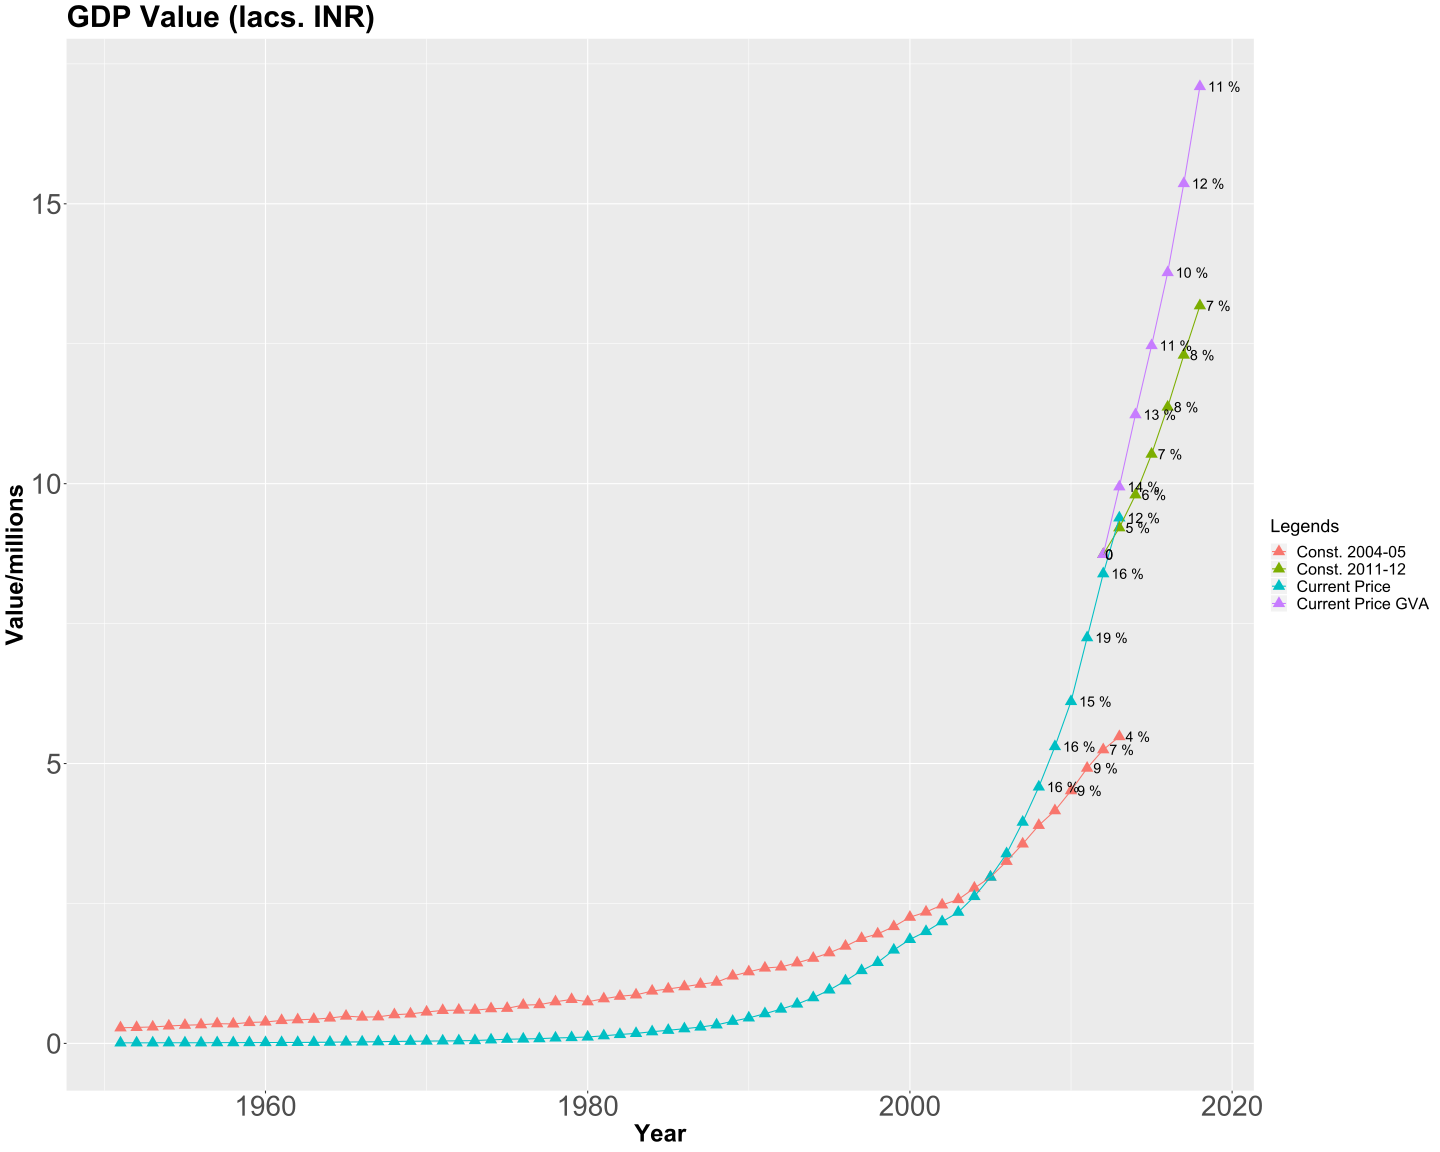
\includegraphics{GDP_India_files/figure-latex/GDP Plots-1.svg}

\hypertarget{analysis-2-gdp-value-trade-deficit}{%
\subsection{Analysis 2: GDP value \& Trade
Deficit}\label{analysis-2-gdp-value-trade-deficit}}

The below chart shows GDP, Import, Export \& Trade deficit against four
different price basis viz., constant 2004-05, constant 2011-12, current
price \& current price GVA. The percentage value on each point indicates
the YoY growth. The values from the year 2001 to 2018 are plotted in
this chart.

\begin{itemize}
\item
  Look at the chart ``constant 2011-12'' - The gap between import \&
  export is low in 2014, 2015, 2016 \& 2017. Corresponding to these
  years, the GDP growth is more compared to other year growth.
\item
  Similarly on the chart ``constant 2004-05'' the gap between imports \&
  export is less during 2006, 2007, 2008, 2010 \& 2011. Corresponding to
  these years, the GDP growth is more compared to other years.
\end{itemize}

\begin{Shaded}
\begin{Highlighting}[]
\NormalTok{GDP_TD_}\DecValTok{2004}\NormalTok{ <-}\StringTok{ }\KeywordTok{select}\NormalTok{(GDP_}\DecValTok{2004}\NormalTok{, year, Base.Price, GDP, Trade.Deficit, Import, Export)}
\NormalTok{GDP_TD_}\DecValTok{2004}\NormalTok{_melt <-}\StringTok{ }\KeywordTok{melt}\NormalTok{(GDP_TD_}\DecValTok{2004}\NormalTok{, }\KeywordTok{c}\NormalTok{(}\StringTok{"year"}\NormalTok{, }\StringTok{"Base.Price"}\NormalTok{))}
\NormalTok{GDP_TD_}\DecValTok{2004}\NormalTok{_melt_filter <-}\StringTok{ }\NormalTok{GDP_TD_}\DecValTok{2004}\NormalTok{_melt }\OperatorTok\StringTok{ }\KeywordTok{filter}\NormalTok{(year }\OperatorTok\StringTok{ }\DecValTok{2001}\OperatorTok{:}\DecValTok{2012}\NormalTok{)}
\NormalTok{GDP_TD_}\DecValTok{2004}\NormalTok{_melt_filter}\OperatorTok{$}\NormalTok{value <-}\StringTok{ }\NormalTok{GDP_TD_}\DecValTok{2004}\NormalTok{_melt_filter}\OperatorTok{$}\NormalTok{value}\OperatorTok{/}\DecValTok{1000000}
\NormalTok{GDP_TD_}\DecValTok{2004}\NormalTok{_melt_filter}\OperatorTok{$}\NormalTok{vj <-}\StringTok{ }\KeywordTok{rep}\NormalTok{(}\KeywordTok{c}\NormalTok{(}\OperatorTok{-}\DecValTok{1}\NormalTok{,}\DecValTok{1}\NormalTok{), }\DataTypeTok{length.out=}\KeywordTok{nrow}\NormalTok{(GDP_TD_}\DecValTok{2004}\NormalTok{_melt_filter))}
\ControlFlowTok{for}\NormalTok{(i }\ControlFlowTok{in} \DecValTok{1}\OperatorTok{:}\KeywordTok{nrow}\NormalTok{(GDP_TD_}\DecValTok{2004}\NormalTok{_melt_filter))\{}
    \ControlFlowTok{if}\NormalTok{(GDP_TD_}\DecValTok{2004}\NormalTok{_melt_filter}\OperatorTok{$}\NormalTok{year[i]}\OperatorTok{==}\DecValTok{2001}\NormalTok{)\{GDP_TD_}\DecValTok{2004}\NormalTok{_melt_filter}\OperatorTok{$}\NormalTok{Percent_Change[i] <-}\StringTok{ }\DecValTok{0}\NormalTok{\}}
    \ControlFlowTok{else}\NormalTok{\{GDP_TD_}\DecValTok{2004}\NormalTok{_melt_filter}\OperatorTok{$}\NormalTok{Percent_Change[i] <-}\StringTok{ }\KeywordTok{sprintf}\NormalTok{(}\StringTok{"%.0f %%"}\NormalTok{, }\DecValTok{100}\OperatorTok{*}\NormalTok{((GDP_TD_}\DecValTok{2004}\NormalTok{_melt_filter}\OperatorTok{$}\NormalTok{value[i] }\OperatorTok{-}\NormalTok{GDP_TD_}\DecValTok{2004}\NormalTok{_melt_filter}\OperatorTok{$}\NormalTok{value[i}\DecValTok{-1}\NormalTok{]) }\OperatorTok{/}\StringTok{ }\NormalTok{GDP_TD_}\DecValTok{2004}\NormalTok{_melt_filter}\OperatorTok{$}\NormalTok{value[i}\DecValTok{-1}\NormalTok{]))\}}
\NormalTok{\}}
\end{Highlighting}
\end{Shaded}

\begin{Shaded}
\begin{Highlighting}[]
\NormalTok{GDP_TD_}\DecValTok{2011}\NormalTok{ <-}\StringTok{ }\KeywordTok{select}\NormalTok{(GDP_}\DecValTok{2011}\NormalTok{, year, Base.Price, GDP, Trade.Deficit, Import, Export)}
\NormalTok{GDP_TD_}\DecValTok{2011}\NormalTok{_melt <-}\StringTok{ }\KeywordTok{melt}\NormalTok{(GDP_TD_}\DecValTok{2011}\NormalTok{, }\KeywordTok{c}\NormalTok{(}\StringTok{"year"}\NormalTok{, }\StringTok{"Base.Price"}\NormalTok{))}
\NormalTok{GDP_TD_}\DecValTok{2011}\NormalTok{_melt}\OperatorTok{$}\NormalTok{value <-}\StringTok{ }\NormalTok{GDP_TD_}\DecValTok{2011}\NormalTok{_melt}\OperatorTok{$}\NormalTok{value}\OperatorTok{/}\DecValTok{1000000}
\NormalTok{GDP_TD_}\DecValTok{2011}\NormalTok{_melt}\OperatorTok{$}\NormalTok{vj <-}\StringTok{ }\KeywordTok{rep}\NormalTok{(}\KeywordTok{c}\NormalTok{(}\OperatorTok{-}\DecValTok{1}\NormalTok{,}\DecValTok{1}\NormalTok{), }\DataTypeTok{length.out=}\KeywordTok{nrow}\NormalTok{(GDP_TD_}\DecValTok{2011}\NormalTok{_melt))}
\ControlFlowTok{for}\NormalTok{(i }\ControlFlowTok{in} \DecValTok{1}\OperatorTok{:}\KeywordTok{nrow}\NormalTok{(GDP_TD_}\DecValTok{2011}\NormalTok{_melt))\{}
 \ControlFlowTok{if}\NormalTok{(GDP_TD_}\DecValTok{2011}\NormalTok{_melt}\OperatorTok{$}\NormalTok{year[i]}\OperatorTok{==}\DecValTok{2012}\NormalTok{)\{GDP_TD_}\DecValTok{2011}\NormalTok{_melt}\OperatorTok{$}\NormalTok{Percent_Change[i] <-}\StringTok{ }\DecValTok{0}\NormalTok{\}}
 \ControlFlowTok{else}\NormalTok{\{GDP_TD_}\DecValTok{2011}\NormalTok{_melt}\OperatorTok{$}\NormalTok{Percent_Change[i] <-}\StringTok{ }\KeywordTok{sprintf}\NormalTok{(}\StringTok{"%.0f %%"}\NormalTok{, }\DecValTok{100}\OperatorTok{*}\NormalTok{((GDP_TD_}\DecValTok{2011}\NormalTok{_melt}\OperatorTok{$}\NormalTok{value[i] }\OperatorTok{-}\NormalTok{GDP_TD_}\DecValTok{2011}\NormalTok{_melt}\OperatorTok{$}\NormalTok{value[i}\DecValTok{-1}\NormalTok{]) }\OperatorTok{/}\StringTok{ }\NormalTok{GDP_TD_}\DecValTok{2011}\NormalTok{_melt}\OperatorTok{$}\NormalTok{value[i}\DecValTok{-1}\NormalTok{]))\}}
\NormalTok{\}}
\end{Highlighting}
\end{Shaded}

\begin{Shaded}
\begin{Highlighting}[]
\NormalTok{GDP_TD_}\DecValTok{2004}\NormalTok{_plot <-}\StringTok{ }\KeywordTok{ggplot}\NormalTok{(GDP_TD_}\DecValTok{2004}\NormalTok{_melt_filter, }\KeywordTok{aes}\NormalTok{(year, value))}\OperatorTok{+}\KeywordTok{geom_point}\NormalTok{(}\KeywordTok{aes}\NormalTok{(}\DataTypeTok{color=}\NormalTok{GDP_TD_}\DecValTok{2004}\NormalTok{_melt_filter}\OperatorTok{$}\NormalTok{variable), }\DataTypeTok{size=}\DecValTok{4}\NormalTok{, }\DataTypeTok{pch=}\DecValTok{17}\NormalTok{)}\OperatorTok{+}\KeywordTok{facet_grid}\NormalTok{(.}\OperatorTok{~}\NormalTok{GDP_TD_}\DecValTok{2004}\NormalTok{_melt_filter}\OperatorTok{$}\NormalTok{Base.Price)}\OperatorTok{+}\KeywordTok{geom_line}\NormalTok{(}\KeywordTok{aes}\NormalTok{(}\DataTypeTok{color =}\NormalTok{ GDP_TD_}\DecValTok{2004}\NormalTok{_melt_filter}\OperatorTok{$}\NormalTok{variable)) }\OperatorTok{+}\KeywordTok{labs}\NormalTok{(}\DataTypeTok{x=}\StringTok{"Year"}\NormalTok{, }\DataTypeTok{y=}\StringTok{"Value/millions"}\NormalTok{, }\DataTypeTok{title=}\StringTok{"GDP Value & Trade Deficit (lacs. INR)"}\NormalTok{, }\DataTypeTok{color =} \StringTok{"Legends"}\NormalTok{)}\OperatorTok{+}\StringTok{ }\KeywordTok{geom_text}\NormalTok{(}\KeywordTok{aes}\NormalTok{(}\DataTypeTok{label =} \KeywordTok{ifelse}\NormalTok{(GDP_TD_}\DecValTok{2004}\NormalTok{_melt_filter}\OperatorTok{$}\NormalTok{value }\OperatorTok{>}\StringTok{ }\DecValTok{0}\NormalTok{, }\KeywordTok{as.character}\NormalTok{(GDP_TD_}\DecValTok{2004}\NormalTok{_melt_filter}\OperatorTok{$}\NormalTok{Percent_Change), }\StringTok{''}\NormalTok{)), }\DataTypeTok{hjust =} \DecValTok{0}\NormalTok{, }\DataTypeTok{vjust =}\NormalTok{ GDP_TD_}\DecValTok{2004}\NormalTok{_melt_filter}\OperatorTok{$}\NormalTok{vj, }\DataTypeTok{size =} \DecValTok{5}\NormalTok{)}\OperatorTok{+}\StringTok{ }\NormalTok{plot_theme }\OperatorTok{+}\StringTok{ }\KeywordTok{scale_x_continuous}\NormalTok{(}\DataTypeTok{breaks =} \KeywordTok{round}\NormalTok{(}\KeywordTok{seq}\NormalTok{(}\KeywordTok{min}\NormalTok{(GDP_TD_}\DecValTok{2004}\NormalTok{_melt_filter}\OperatorTok{$}\NormalTok{year), }\KeywordTok{max}\NormalTok{(GDP_TD_}\DecValTok{2004}\NormalTok{_melt_filter}\OperatorTok{$}\NormalTok{year), }\DataTypeTok{by =} \DecValTok{2}\NormalTok{),}\DecValTok{1}\NormalTok{))}

\NormalTok{GDP_TD_}\DecValTok{2011}\NormalTok{_plot <-}\StringTok{ }\KeywordTok{ggplot}\NormalTok{(GDP_TD_}\DecValTok{2011}\NormalTok{_melt, }\KeywordTok{aes}\NormalTok{(year, value))}\OperatorTok{+}\KeywordTok{geom_point}\NormalTok{(}\KeywordTok{aes}\NormalTok{(}\DataTypeTok{color=}\NormalTok{GDP_TD_}\DecValTok{2011}\NormalTok{_melt}\OperatorTok{$}\NormalTok{variable), }\DataTypeTok{size=}\DecValTok{4}\NormalTok{, }\DataTypeTok{pch=}\DecValTok{17}\NormalTok{)}\OperatorTok{+}\KeywordTok{facet_grid}\NormalTok{(.}\OperatorTok{~}\NormalTok{GDP_TD_}\DecValTok{2011}\NormalTok{_melt}\OperatorTok{$}\NormalTok{Base.Price)}\OperatorTok{+}\KeywordTok{geom_line}\NormalTok{(}\KeywordTok{aes}\NormalTok{(}\DataTypeTok{color =}\NormalTok{ GDP_TD_}\DecValTok{2011}\NormalTok{_melt}\OperatorTok{$}\NormalTok{variable)) }\OperatorTok{+}\KeywordTok{labs}\NormalTok{(}\DataTypeTok{x=}\StringTok{"Year"}\NormalTok{, }\DataTypeTok{y=}\StringTok{"Value/millions"}\NormalTok{, }\DataTypeTok{color =} \StringTok{"Legends"}\NormalTok{)}\OperatorTok{+}\StringTok{ }\KeywordTok{geom_text}\NormalTok{(}\KeywordTok{aes}\NormalTok{(}\DataTypeTok{label =} \KeywordTok{ifelse}\NormalTok{(GDP_TD_}\DecValTok{2011}\NormalTok{_melt}\OperatorTok{$}\NormalTok{value }\OperatorTok{>}\StringTok{ }\DecValTok{0}\NormalTok{, }\KeywordTok{as.character}\NormalTok{(GDP_TD_}\DecValTok{2011}\NormalTok{_melt}\OperatorTok{$}\NormalTok{Percent_Change), }\StringTok{''}\NormalTok{)), }\DataTypeTok{hjust =} \DecValTok{0}\NormalTok{, }\DataTypeTok{vjust =}\NormalTok{ GDP_TD_}\DecValTok{2011}\NormalTok{_melt}\OperatorTok{$}\NormalTok{vj, }\DataTypeTok{size =} \DecValTok{5}\NormalTok{)}\OperatorTok{+}\StringTok{ }\NormalTok{plot_theme}

\KeywordTok{plot_grid}\NormalTok{(GDP_TD_}\DecValTok{2004}\NormalTok{_plot, GDP_TD_}\DecValTok{2011}\NormalTok{_plot, }\DataTypeTok{nrow =} \DecValTok{2}\NormalTok{)}
\end{Highlighting}
\end{Shaded}

\includegraphics{GDP_India_files/figure-latex/GDP \& trade deficit plot-1.svg}

\hypertarget{analysis-3-gdp-of-agricultural-products-and-its-contribution-to-total-gdp}{%
\subsection{Analysis 3: GDP of Agricultural products and its
Contribution to total
GDP}\label{analysis-3-gdp-of-agricultural-products-and-its-contribution-to-total-gdp}}

The below chart shows the total GDP \& GDP of agricultural products. The
percentage value given over each point of ``GDP\_AGRI'' \& ``GVA\_AGRI''
is the percentage contribution of agricultural products to the overall
GDP. From 2011 the GDP value is calculated based on the GVA basis. The
values from the year 2001 to 2018 are plotted in this chart.

\begin{itemize}
\tightlist
\item
  In ``const 2004-05'', ``current price'' \& ``const 2011-12'' chart the
  GDP value of agricultural products is having positive growth, but at
  the same time, its contribution to the overall GDP is reducing year on
  year.
\item
  In ``current price GVA'' chart both the value and its contribution to
  overall GDP of agricultural product is having a negative growth.
\end{itemize}

\begin{Shaded}
\begin{Highlighting}[]
\NormalTok{GDP_Agri_}\DecValTok{2004}\NormalTok{ <-}\StringTok{ }\KeywordTok{select}\NormalTok{(GDP_}\DecValTok{2004}\NormalTok{, }\StringTok{"year"}\NormalTok{, }\StringTok{"Base.Price"}\NormalTok{, }\StringTok{"GDP"}\NormalTok{, }\StringTok{"GDP_AGRI"}\NormalTok{)}
\NormalTok{GDP_Agri_}\DecValTok{2004}\NormalTok{_filter <-}\StringTok{ }\NormalTok{GDP_Agri_}\DecValTok{2004} \OperatorTok\StringTok{ }\KeywordTok{filter}\NormalTok{(year }\OperatorTok\StringTok{ }\DecValTok{2001}\OperatorTok{:}\DecValTok{2012}\NormalTok{)}
\ControlFlowTok{for}\NormalTok{(i }\ControlFlowTok{in} \DecValTok{1}\OperatorTok{:}\KeywordTok{nrow}\NormalTok{(GDP_Agri_}\DecValTok{2004}\NormalTok{_filter))\{}
 \ControlFlowTok{if}\NormalTok{(GDP_Agri_}\DecValTok{2004}\NormalTok{_filter}\OperatorTok{$}\NormalTok{year[i]}\OperatorTok{==}\DecValTok{2001}\NormalTok{)\{GDP_Agri_}\DecValTok{2004}\NormalTok{_filter}\OperatorTok{$}\NormalTok{Percent_Change[i] <-}\StringTok{ }\DecValTok{0}\NormalTok{\}}
 \ControlFlowTok{else}\NormalTok{\{GDP_Agri_}\DecValTok{2004}\NormalTok{_filter}\OperatorTok{$}\NormalTok{Percent_Change[i] <-}\StringTok{ }\KeywordTok{round}\NormalTok{(}\DecValTok{100}\OperatorTok{*}\NormalTok{GDP_Agri_}\DecValTok{2004}\NormalTok{_filter}\OperatorTok{$}\NormalTok{GDP_AGRI[i]}\OperatorTok{/}\NormalTok{GDP_Agri_}\DecValTok{2004}\NormalTok{_filter}\OperatorTok{$}\NormalTok{GDP[i], }\DataTypeTok{digits =} \DecValTok{2}\NormalTok{)\}}
\NormalTok{\}}
\NormalTok{GDP_Agri_}\DecValTok{2004}\NormalTok{_melt <-}\StringTok{ }\KeywordTok{melt}\NormalTok{(GDP_Agri_}\DecValTok{2004}\NormalTok{_filter, }\KeywordTok{c}\NormalTok{(}\StringTok{"year"}\NormalTok{, }\StringTok{"Base.Price"}\NormalTok{, }\StringTok{"Percent_Change"}\NormalTok{))}
\NormalTok{GDP_Agri_}\DecValTok{2004}\NormalTok{_melt}\OperatorTok{$}\NormalTok{value <-}\StringTok{ }\NormalTok{GDP_Agri_}\DecValTok{2004}\NormalTok{_melt}\OperatorTok{$}\NormalTok{value}\OperatorTok{/}\DecValTok{1000000}

\NormalTok{GDP_Agri_}\DecValTok{2011}\NormalTok{ <-}\StringTok{ }\KeywordTok{select}\NormalTok{(GDP_}\DecValTok{2011}\NormalTok{, }\StringTok{"year"}\NormalTok{, }\StringTok{"Base.Price"}\NormalTok{, }\StringTok{"GDP"}\NormalTok{, }\StringTok{"GVA_AGRI"}\NormalTok{)}
\CommentTok{#GDP_Agri_2011_filter <- GDP_Agri_2011 %>% filter(year %in% 2001:2012)}
\ControlFlowTok{for}\NormalTok{(i }\ControlFlowTok{in} \DecValTok{1}\OperatorTok{:}\KeywordTok{nrow}\NormalTok{(GDP_Agri_}\DecValTok{2011}\NormalTok{))\{}
 \ControlFlowTok{if}\NormalTok{(GDP_Agri_}\DecValTok{2011}\OperatorTok{$}\NormalTok{year[i]}\OperatorTok{==}\DecValTok{2012}\NormalTok{)\{GDP_Agri_}\DecValTok{2011}\OperatorTok{$}\NormalTok{Percent_Change[i] <-}\StringTok{ }\DecValTok{0}\NormalTok{\}}
 \ControlFlowTok{else}\NormalTok{\{GDP_Agri_}\DecValTok{2011}\OperatorTok{$}\NormalTok{Percent_Change[i] <-}\StringTok{ }\KeywordTok{round}\NormalTok{(}\DecValTok{100}\OperatorTok{*}\NormalTok{GDP_Agri_}\DecValTok{2011}\OperatorTok{$}\NormalTok{GVA_AGRI[i]}\OperatorTok{/}\NormalTok{GDP_Agri_}\DecValTok{2011}\OperatorTok{$}\NormalTok{GDP[i], }\DataTypeTok{digits =} \DecValTok{2}\NormalTok{)\}}
\NormalTok{\}}
\NormalTok{GDP_Agri_}\DecValTok{2011}\NormalTok{_melt <-}\StringTok{ }\KeywordTok{melt}\NormalTok{(GDP_Agri_}\DecValTok{2011}\NormalTok{, }\KeywordTok{c}\NormalTok{(}\StringTok{"year"}\NormalTok{, }\StringTok{"Base.Price"}\NormalTok{, }\StringTok{"Percent_Change"}\NormalTok{))}
\NormalTok{GDP_Agri_}\DecValTok{2011}\NormalTok{_melt}\OperatorTok{$}\NormalTok{value <-}\StringTok{ }\NormalTok{GDP_Agri_}\DecValTok{2011}\NormalTok{_melt}\OperatorTok{$}\NormalTok{value}\OperatorTok{/}\DecValTok{1000000}
\end{Highlighting}
\end{Shaded}

\begin{Shaded}
\begin{Highlighting}[]
\NormalTok{GDP_Agri_}\DecValTok{2004}\NormalTok{_melt}\OperatorTok{$}\NormalTok{vj <-}\StringTok{ }\KeywordTok{rep}\NormalTok{(}\KeywordTok{c}\NormalTok{(}\OperatorTok{-}\DecValTok{1}\NormalTok{,}\DecValTok{1}\NormalTok{), }\DataTypeTok{length.out=}\KeywordTok{nrow}\NormalTok{(GDP_Agri_}\DecValTok{2004}\NormalTok{_melt))}
\NormalTok{GDP_Agri_}\DecValTok{2011}\NormalTok{_melt}\OperatorTok{$}\NormalTok{vj <-}\StringTok{ }\KeywordTok{rep}\NormalTok{(}\KeywordTok{c}\NormalTok{(}\OperatorTok{-}\DecValTok{1}\NormalTok{,}\DecValTok{1}\NormalTok{), }\DataTypeTok{length.out=}\KeywordTok{nrow}\NormalTok{(GDP_Agri_}\DecValTok{2011}\NormalTok{_melt))}

\NormalTok{GDP_Agri_plot_}\DecValTok{2004}\NormalTok{ <-}\StringTok{ }\KeywordTok{ggplot}\NormalTok{(GDP_Agri_}\DecValTok{2004}\NormalTok{_melt, }\KeywordTok{aes}\NormalTok{(year, value))}\OperatorTok{+}\StringTok{ }\KeywordTok{geom_point}\NormalTok{(}\KeywordTok{aes}\NormalTok{(}\DataTypeTok{color=}\NormalTok{variable), }\DataTypeTok{size=}\DecValTok{4}\NormalTok{, }\DataTypeTok{pch=}\DecValTok{17}\NormalTok{)}\OperatorTok{+}\StringTok{ }\KeywordTok{facet_grid}\NormalTok{(.}\OperatorTok{~}\NormalTok{Base.Price)}\OperatorTok{+}\StringTok{ }\KeywordTok{geom_line}\NormalTok{(}\KeywordTok{aes}\NormalTok{(}\DataTypeTok{color =}\NormalTok{ GDP_Agri_}\DecValTok{2004}\NormalTok{_melt}\OperatorTok{$}\NormalTok{variable))}\OperatorTok{+}\StringTok{ }\KeywordTok{geom_text}\NormalTok{(}\KeywordTok{aes}\NormalTok{(}\DataTypeTok{label=} \KeywordTok{ifelse}\NormalTok{(GDP_Agri_}\DecValTok{2004}\NormalTok{_melt}\OperatorTok{$}\NormalTok{variable }\OperatorTok{==}\StringTok{ "GDP_AGRI"}\NormalTok{, GDP_Agri_}\DecValTok{2004}\NormalTok{_melt}\OperatorTok{$}\NormalTok{Percent_Change, }\StringTok{''}\NormalTok{)),}\DataTypeTok{hjust =} \DecValTok{0}\NormalTok{, }\DataTypeTok{vjust =}\NormalTok{ GDP_Agri_}\DecValTok{2004}\NormalTok{_melt}\OperatorTok{$}\NormalTok{vj, }\DataTypeTok{size =} \DecValTok{5}\NormalTok{)}\OperatorTok{+}\StringTok{ }\KeywordTok{labs}\NormalTok{(}\DataTypeTok{x=}\StringTok{"Year"}\NormalTok{, }\DataTypeTok{y=}\StringTok{"Value/millions"}\NormalTok{, }\DataTypeTok{title=}\StringTok{"GDP & GDP of Agricutural Products (lacs. INR)"}\NormalTok{, }\DataTypeTok{color =} \StringTok{"Legends"}\NormalTok{) }\OperatorTok{+}\StringTok{ }\NormalTok{plot_theme }\OperatorTok{+}\StringTok{ }\KeywordTok{scale_x_continuous}\NormalTok{(}\DataTypeTok{breaks =} \KeywordTok{round}\NormalTok{(}\KeywordTok{seq}\NormalTok{(}\KeywordTok{min}\NormalTok{(GDP_Agri_}\DecValTok{2004}\NormalTok{_melt}\OperatorTok{$}\NormalTok{year), }\KeywordTok{max}\NormalTok{(GDP_Agri_}\DecValTok{2004}\NormalTok{_melt}\OperatorTok{$}\NormalTok{year), }\DataTypeTok{by =} \DecValTok{2}\NormalTok{),}\DecValTok{1}\NormalTok{))}

\NormalTok{GDP_Agri_plot_}\DecValTok{2011}\NormalTok{ <-}\StringTok{ }\KeywordTok{ggplot}\NormalTok{(GDP_Agri_}\DecValTok{2011}\NormalTok{_melt, }\KeywordTok{aes}\NormalTok{(year, value))}\OperatorTok{+}\StringTok{ }\KeywordTok{geom_point}\NormalTok{(}\KeywordTok{aes}\NormalTok{(}\DataTypeTok{color=}\NormalTok{variable), }\DataTypeTok{size=}\DecValTok{4}\NormalTok{, }\DataTypeTok{pch=}\DecValTok{17}\NormalTok{)}\OperatorTok{+}\StringTok{ }\KeywordTok{facet_grid}\NormalTok{(.}\OperatorTok{~}\NormalTok{Base.Price)}\OperatorTok{+}\StringTok{ }\KeywordTok{geom_line}\NormalTok{(}\KeywordTok{aes}\NormalTok{(}\DataTypeTok{color =}\NormalTok{ GDP_Agri_}\DecValTok{2011}\NormalTok{_melt}\OperatorTok{$}\NormalTok{variable))}\OperatorTok{+}\StringTok{ }\KeywordTok{geom_text}\NormalTok{(}\KeywordTok{aes}\NormalTok{(}\DataTypeTok{label=} \KeywordTok{ifelse}\NormalTok{(GDP_Agri_}\DecValTok{2011}\NormalTok{_melt}\OperatorTok{$}\NormalTok{variable }\OperatorTok{==}\StringTok{ "GVA_AGRI"}\NormalTok{, GDP_Agri_}\DecValTok{2011}\NormalTok{_melt}\OperatorTok{$}\NormalTok{Percent_Change, }\StringTok{''}\NormalTok{)),}\DataTypeTok{hjust =} \DecValTok{0}\NormalTok{, }\DataTypeTok{vjust =}\NormalTok{ GDP_Agri_}\DecValTok{2011}\NormalTok{_melt}\OperatorTok{$}\NormalTok{vj, }\DataTypeTok{size =} \DecValTok{5}\NormalTok{)}\OperatorTok{+}\StringTok{ }\KeywordTok{labs}\NormalTok{(}\DataTypeTok{x=}\StringTok{"Year"}\NormalTok{, }\DataTypeTok{y=}\StringTok{"Value/millions"}\NormalTok{, }\DataTypeTok{color =} \StringTok{"Legends"}\NormalTok{) }\OperatorTok{+}\StringTok{ }\NormalTok{plot_theme }\OperatorTok{+}\StringTok{ }\KeywordTok{scale_x_continuous}\NormalTok{(}\DataTypeTok{breaks =} \KeywordTok{round}\NormalTok{(}\KeywordTok{seq}\NormalTok{(}\KeywordTok{min}\NormalTok{(GDP_Agri_}\DecValTok{2011}\NormalTok{_melt}\OperatorTok{$}\NormalTok{year), }\KeywordTok{max}\NormalTok{(GDP_Agri_}\DecValTok{2011}\NormalTok{_melt}\OperatorTok{$}\NormalTok{year), }\DataTypeTok{by =} \DecValTok{2}\NormalTok{),}\DecValTok{1}\NormalTok{))}

\KeywordTok{plot_grid}\NormalTok{(GDP_Agri_plot_}\DecValTok{2004}\NormalTok{, GDP_Agri_plot_}\DecValTok{2011}\NormalTok{, }\DataTypeTok{nrow =} \DecValTok{2}\NormalTok{)}
\end{Highlighting}
\end{Shaded}

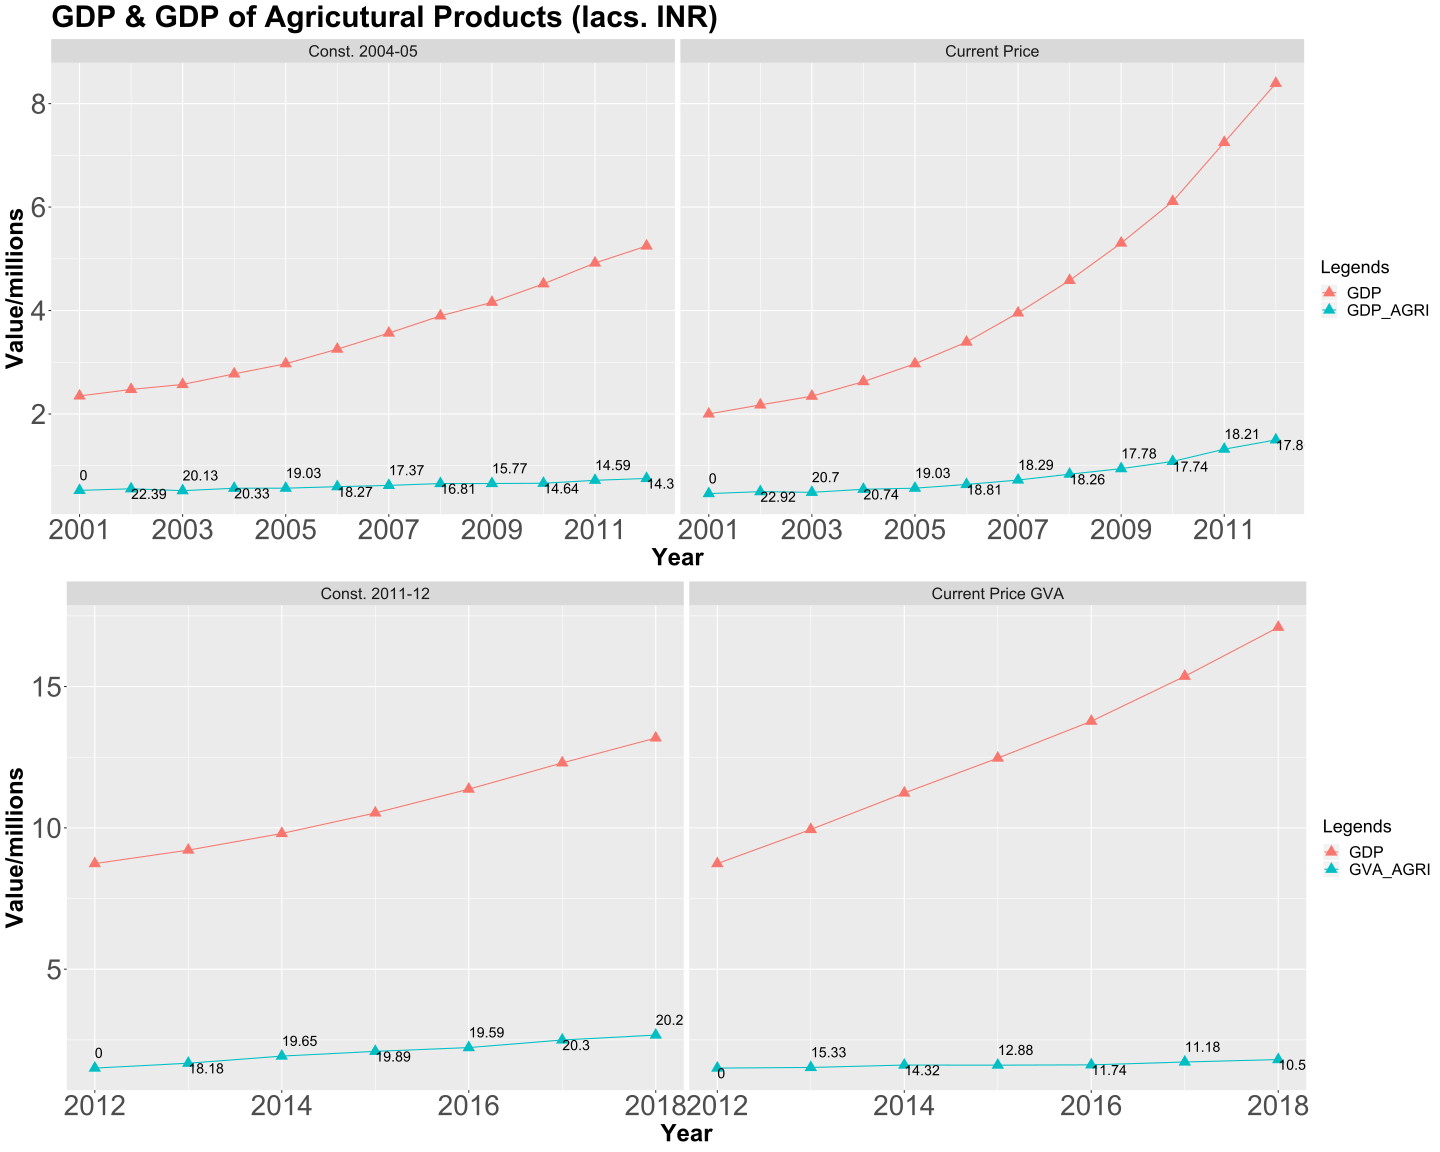
\includegraphics{GDP_India_files/figure-latex/Plot of Agri products-1.svg}


\end{document}
